\documentclass{beamer}
\usepackage[utf8]{inputenc}
\usepackage{graphics}
\usepackage{url}
\usepackage{pstricks}

\usetheme{Malmoe}
% \usetheme{CambridgeUS}
\usecolortheme{beaver}
\useoutertheme{infolines}

\title[Copier/coller multi-plateforme]{Étude du problème de copier/coller
  multi-plateformes et implémentation d'une solution}
\author{Maëlick Claes}
\institute[UMons - M1 Info]{
\includegraphics[width=100px]{umons}\\
Faculté des Sciences - Première année du Master en Sciences Informatiques}
\date{24 juin 2011}

\begin{document}

\AtBeginSection[]
{
  \begin{frame}<beamer>
    \frametitle{Plan}
    \tableofcontents[currentsection, currentsubsection]
  \end{frame}
}
\AtBeginSubsection[]
{
  \begin{frame}<beamer>
    \frametitle{Plan}
    \tableofcontents[currentsection,currentsubsection]
  \end{frame}
}

\beamertemplatetransparentcovered

\begin{frame}
  \titlepage
\end{frame}

\begin{frame}{Table des matières}
  \tableofcontents
\end{frame}

\section{Introduction}
\begin{frame}{Introduction}
  \begin{block}{Copier/coller multi-écrans}
    \center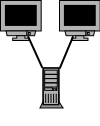
\includegraphics{ccmp1}
  \end{block}
\end{frame}

\begin{frame}{Introduction}
  \begin{block}{Copier/coller multi-plateformes}
    \center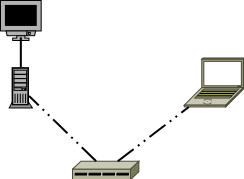
\includegraphics[width=200px]{ccmp2}
  \end{block}
\end{frame}

\section{Solutions existantes}
\begin{frame}{Solutions lourdes}
  \begin{itemize}
  \item Échange d'e-mails
  \item Serveur FTP
  \item Partage de fichiers
  \item Outils de travail collaboratif
  \item Partage de bureaux:
    \begin{itemize}
    \item Remote Desktop Services
    \item VNC
    \item Citrix XenApp
    \item NX
    \end{itemize}
  \item ClusterSSH
  \end{itemize}
\end{frame}

\begin{frame}{Solutions légères}
  \begin{itemize}
  \item CL1P
  \item ClipboardMultiSharer
  \item ClipboardShare
  \item The Network Clipboard
  \item Remote Clip
  \end{itemize}
\end{frame}

\begin{frame}{CL1P}
    \begin{description}
    \item[+] HTTPS et choix des utilisateurs
    \item[-] Centralisé
    \item[-] Serveur aux USA
    \item[-] Page web
    \end{description}
  \begin{block}{CL1P en image}
    \center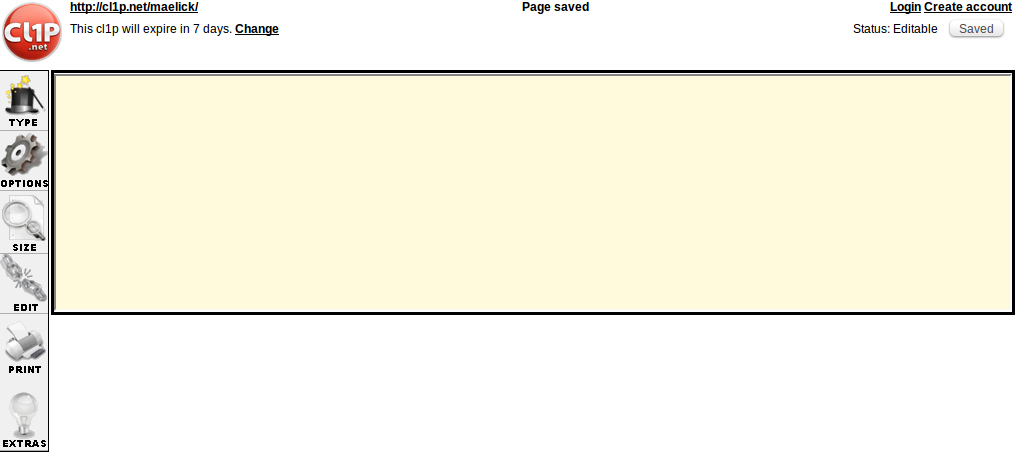
\includegraphics[width=0.6\textwidth]{cl1p}
  \end{block}
\end{frame}

\begin{frame}{ClipboardMultiSharer}
  \begin{description}
  \item[+] JAVA $\Rightarrow$ logiciel portable
  \item[+] Open-source
  \item[-] Partage de fichiers
  \end{description}
  \begin{block}{ClipboardMultiSharer en image}
    \center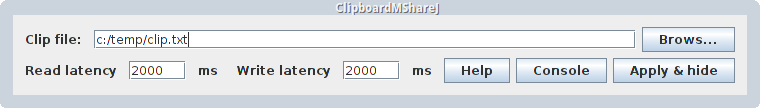
\includegraphics[width=\textwidth]{clipboardmshare}
  \end{block}
\end{frame}

\begin{frame}{ClipboardShare}
  \begin{description}
    \item[+] Architecture P2P décentralisée
    \item[+] Connexion chiffrée et envoyeur de confiance
    \item[-] .NET 3.5 et PNRP
  \end{description}
\end{frame}

\begin{frame}{The Network Clipboard}
  \begin{description}
  \item[+] Open-source
  \item[+] Code source portable en C++
  \item[+] Décentralisé (broadcast)
  \item[-] Pas de sécurité
  \item[-] Qt3
  \end{description}
  \begin{block}{The Network Clipboard en images}
    \center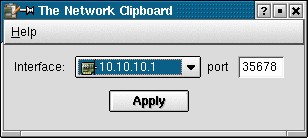
\includegraphics[width=100px]{netclip1}
    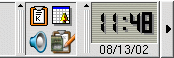
\includegraphics[wdith=50px]{netclip2}
  \end{block}
\end{frame}

\begin{frame}{Remote Clip}
  \begin{description}
  \item[+] SSL et choix des pairs
  \item[+] JAVA $\Rightarrow$ logiciel portable
  \item[-] Dernière version: 10 juillet 2002
  \end{description}
  \begin{block}{Remote Clip en image}
    \center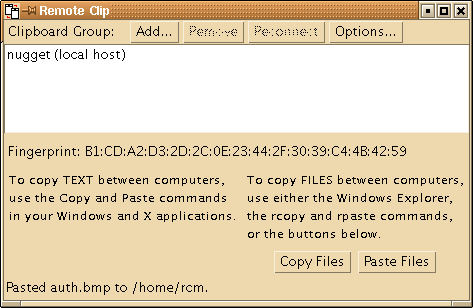
\includegraphics[width=150px]{remoteclip}
  \end{block}
\end{frame}

\section{Clipsync}
\begin{frame}{Rappel}
  \begin{block}{Topologie client-serveur VS topologie peer-to-peer}
    \vspace{1em}
    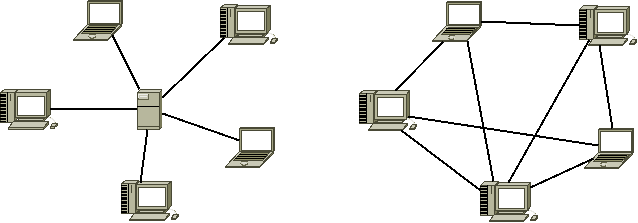
\includegraphics[width=\textwidth]{fig_p2p}
  \end{block}
\end{frame}

\begin{frame}{Broadcast}
  \begin{itemize}
  \item Chaque pair envoie des messages broadcast sur le LAN
  \item Réception d'un message $\Rightarrow$ contacter le pair qui a
    envoyé le message
  \end{itemize}
\end{frame}

\begin{frame}{Authentification}
  \begin{itemize}
  \item Communication chiffrée avec AES-256
  \item Envoi d'un Nonce $\Rightarrow$ Renvoi du Nonce incrémenté
  \item Keep Alive
  \end{itemize}
\end{frame}

\begin{frame}{Envoi du presse-papier}
  \begin{block}{Deux solutions}
    \begin{itemize}
    \item Lorsqu'un copier est effectué:
      \begin{description}
      \item[+] Remote Clip et X Window
      \item[-] Faible tolérance aux erreurs
      \end{description}
    \item Lorsqu'un coller est effectué:
      \begin{description}
      \item[+] Haute tolérance aux erreurs
      \end{description}
    \end{itemize}
  \end{block}
\end{frame}

\begin{frame}{Architecture logicielle}
  \begin{itemize}
  \item Principe KISS (Keep It Simple, Stupid), Philosophie Unix
  \item Client \emph{P2P}: front-end avec le réseau: Clipsync
  \item Clients locaux: front-ends avec l'utilisateurs: Shellclip et GTKClip
  \item Disponibles sur Launchpad: \url{https://launchpad.net/clipsync}
  \end{itemize}
\end{frame}

\section{Perspectives}
\begin{frame}{Fonctionnalités}
  \begin{itemize}
  \item Copier/coller de texte: OK
  \item Copier/coller d'autres types de données (\emph{e.g.} images)
  \item Compression des données
  \item Gestion de l'historique du presse-papier
  \item IPv6
  \item Remplacement du broadcast: \emph{Zeroconf}/\emph{Avahi}/\emph{Bonjour}
  \end{itemize}
\end{frame}

\end{document}
